\documentclass[12pt]{article}
\usepackage[left=12mm, top=0.5in, bottom=0.5in]{geometry}
\usepackage{amsmath}
\usepackage{mathtools}
\usepackage{amssymb}
\usepackage{pifont}
\usepackage{tikz-qtree}
\usepackage{tikz}
\usetikzlibrary{trees}

\newcommand{\cmark}{\ding{51}}%
\newcommand{\xmark}{\ding{55}}%
\newcommand\tab[1][1cm]{\hspace*{#1}}

\begin{document}

\title{Fast Trajectory Replanning}
\author{Austin Bennett, Varun Panchmal}
\maketitle

\section*{Understanding the methods}
	\begin{figure}[!htb]
		\centering
		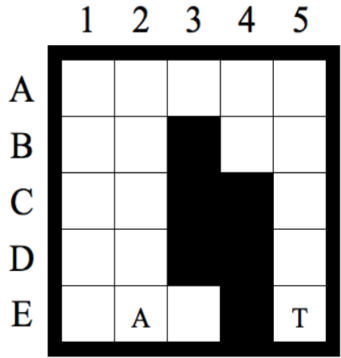
\includegraphics[width=.5\textwidth]{figure_8.png}
		\caption{\label{: }Second Example Search Problem}
	\end{figure}
Throughout the entire Fast Trajectory Replanning assignment, an agent moving in a gridworld is consistently restricted by the following: valid moves are $\in$ \{North, East, South, West\} from the current location, and blocked cells in the gridworld are unknown until they are initially encountered. \\
Consider Figure 1, above, where the starting location is A and the goal location is T. \\
Given that the search algorithm in use is Forward A*, the algorithm will try to expand cells in the cardinal directions while remaining in the bounds of the gridworld. The cells that we end up expanding to are \{E1, D2, E3\}. Our forward A* search will then select the expanded cell with the lowest "cost" or f(n) value.\\
Where f(n) = g(n) + h(n): \\
g(n) = the distance from the start node to node n \\
h(n) = our heuristic function, in this case our heuristic is always the manhattan distance from the goal state to n. \\
Since all of the expanded cells, \{E1, D2, E3\} have the same g(n) value (all of them are 1 cell away from the start) the chosen cell to continue expanding first will be min(h(n)) for n = \{E1, D2, E3\}. Thus our chosen cell to expand first is E3, a poor choice in hindsight, but a necessary choice to ensure that our A star search algorithm always finds the optimal path if it exists. \\ \\
\tab Given a finite gridworld, this project argues that the A star search algorithm will discover the optimal path from the start state to the goal state as long as it is not separated from it by blocked cells and it will discover this optimal path in finite time. The above explanation of why the first move by the A star algorithm in Figure 1 is east is actually extremely good evidence for this argument. The basis of the A star algorithm revolves around the fact that we will always be expanding nodes that are "closest" (closeness is subjective to our heuristic function) to our goal state first up until those paths either find the goal or they hit a blocked path. Given that the goal cell is not completely separated by blocked cells, then the A star algorithm will indeed always find the optimal path in finite time because the algorithm in its worst case will explore every single node in the gridworld. Thus, the algorithm has reached the goal state since we provided the fact that the goal state was not completely blocked off. \\ 
To prove that it can be done in finite time we look at the following figure:
	\begin{figure}[!htb]
		\centering
		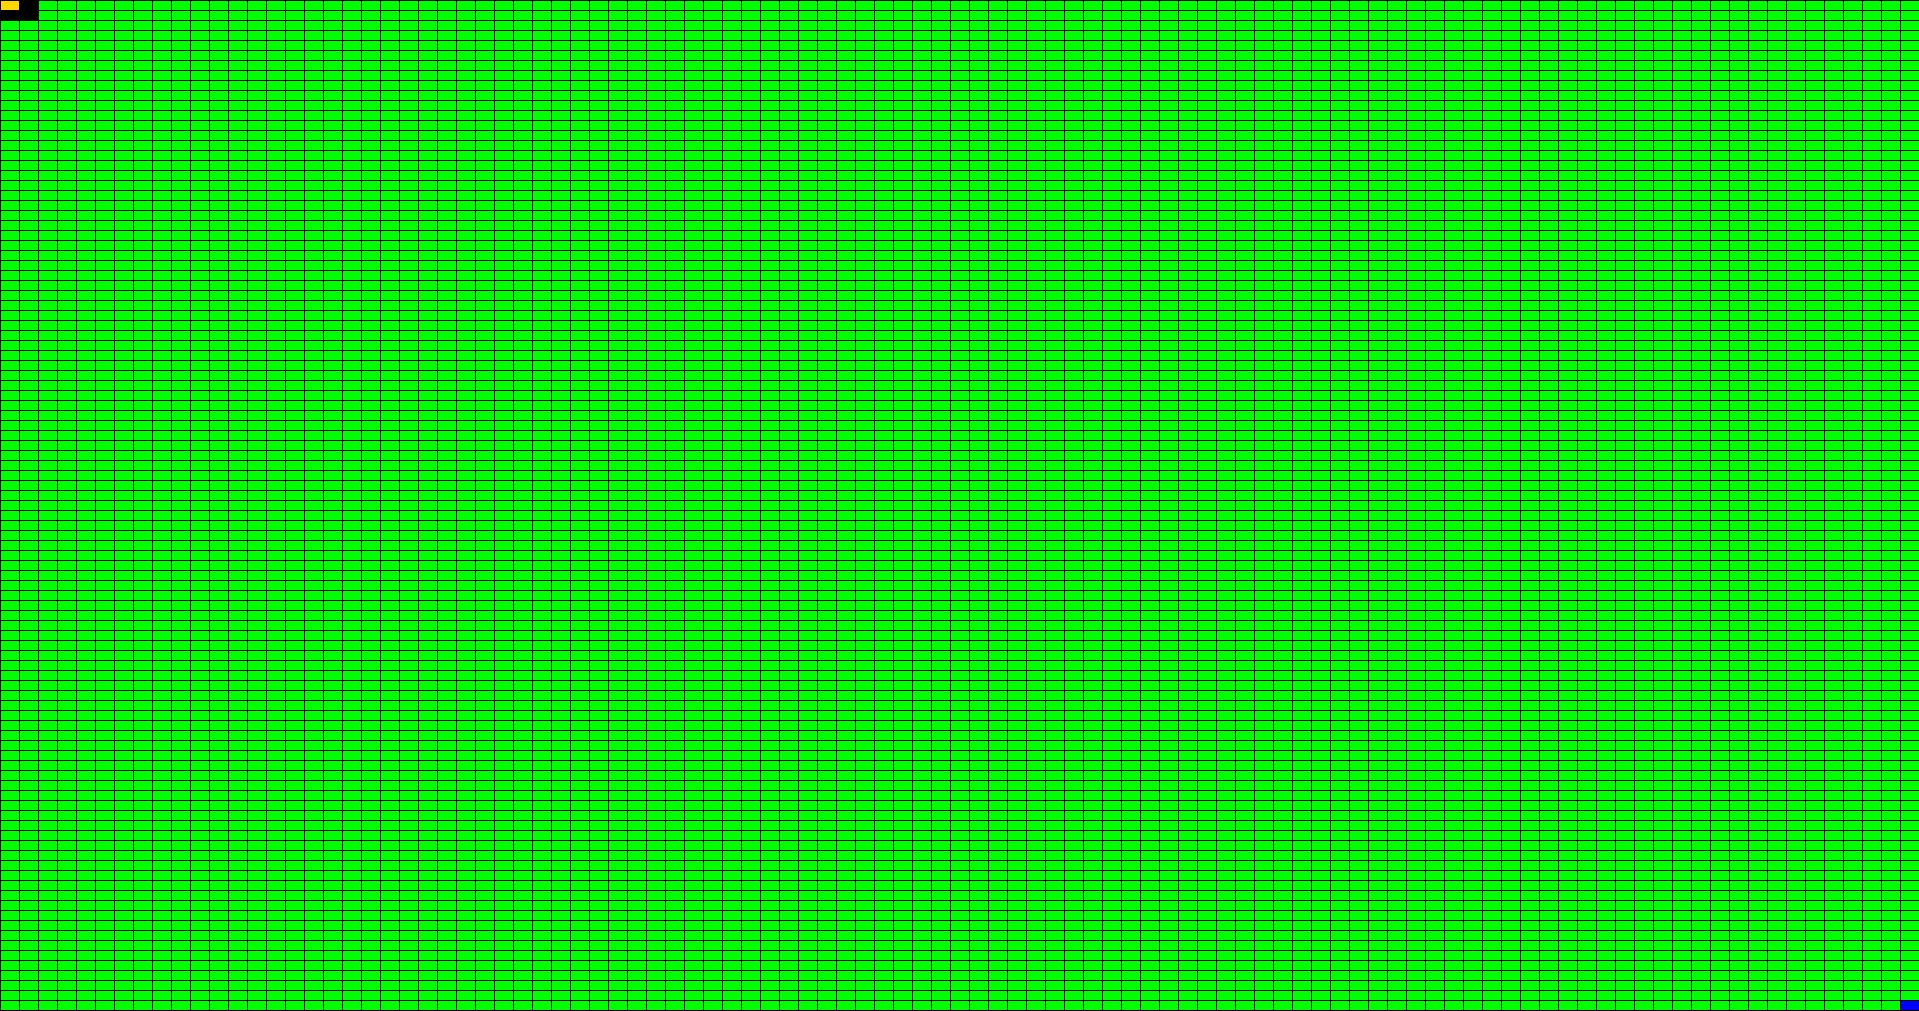
\includegraphics[width=.8\textwidth]{worst_case.png}
		\caption{\label{: }Worst Case Memory Example}
	\end{figure}\\
\tab The goal state is located in the top left and denoted by a yellow cell, surrounded by blocked (black) cells. Our starting cell is in the bottom right and denoted by a blue cell. The green cells in the figure were all unblocked cells that the algorithm has now explored in search of the goal cell. The search algorithm in this case had to explore 101x101 cells (-4 since it can not explore the 3 blocked cells or the goal cell since it is completely blocked off). In any NxN gridworld this will be the worst case in terms of algorithm run time. Thus our number of unblocked cells is 10,197 or NxN-4 for the general case. We can comfortably say then that this process is bounded from above by (NxN-4)$^2$ $\equiv$ our number of unblocked cells squared.\newpage

\section*{The Effects of Ties}
	\begin{figure}[!htb]
		\centering
		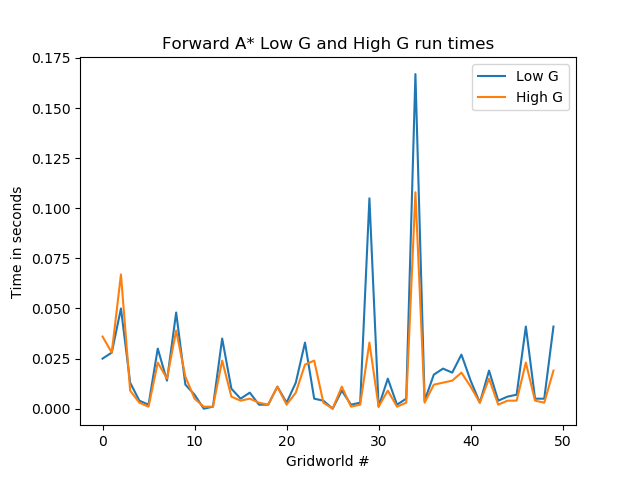
\includegraphics[width=.8\textwidth]{forward_low_vs_high.png}
	\end{figure}
An almost blatant observation that can be concluded from the difference of the high g and low g versions of forward A star is the fact that low g forward A star performs very poor in the cases that the goal state is completely blocked. Low g forward A star search will expand the nodes closer to the start cell in its attempt to establish the best path which is particularly futile when it does all of that groundwork just to find out that the goal state was never reachable. The high g version of forward A star will realize that the goal state is never actually reachable in a much more efficient manner, at least in comparison to low g forward A star.\\
Even in the average case however, high g seems to be marginally to moderately better in almost every gridworld where the goal state is in fact reachable. This should make sense since ideally, you would always prefer to explore paths that are closer to your goal than paths that are further from your goal.
\newpage

\section*{Forward vs. Backward}
	\begin{figure}[!htb]
		\centering
		\includegraphics[width=.8\textwidth]{forward_vs_backward.png}
	\end{figure}
When we introduce backwards A star searching into the equation we start to see some interesting and perhaps surprising results. At first glance it might seem like backwards A star searching is strictly superior. There were 0 cases of backwards A star taking longer than even 0.05 seconds, whereas forwards A star has several above 0.05 seconds and even a 0.17 second run time. It is important to note though that the cases where forward A star took unusally long is because the goal state was completely blocked off and there were no cases that the start state was completely blocked off. In layman's terms: our backwards A star algorithm got lucky.This is extremely important to take note of when considering which algorithm to use in the long run. Ideally, we would test the algorithm on many more random gridworlds if we were trying to decide which algorithm to use in mass scale, for example in a video game.
\newpage

\section*{Heuristics in the Adaptive A*}
\tab The project argues that "the Manhattan distances are consistent in gridworlds in which the agent can move only in the four main compass directions." \\ \\
\tab Foremost, let us establish the definition of consistency: "a heuristic is consistent if its estimate is always less than or equal to the estimated distance from any neighboring vertex to the goal, plus the cost of reaching that neighbor."
	\begin{figure}[!htb]
		\centering
		\includegraphics[width=.4\textwidth]{heuristic_example.png}
		\caption{\label{: }Consistent Heuristic Example}
	\end{figure} \\
Using the manhattan distance heuristic as provided we get: \\
h(A) = 8 \\
h(B) = 7 \\
h(C) = 6 \\
h(A) $\leq$ h(B) + 1 \checkmark \\
h(A) $\leq$ h(C) + 1 \xmark \\
\tab This observation makes sense; with the manhattan distance heuristic if we are moving only laterally or vertically, our distance to the goal cell (T) is going to change by at most 1. Thus, if we are moving closer to the goal cell our heuristic should decrease by 1, but the cost of getting to this new cell was also 1. Therefore, the manhattan distance heuristic is always consistent when restricted to the four main compass directions. We can clearly see that when we release the restriction of movement to the four main compass directions and instead include the diagnols as well; the manhattan distance heuristic is no longer consistent. When moving on a diagnol towards the goal cell we reduce our manhattan distance by 2, because we have completed double the movement that occured when we were restricted to the four main compass directons but our cost stayed the same. \\ \\
\tab Adaptive A* leaves initially consistent h-values consistent even if action costs can increase or decrease. When iterating through the A star search algorithm, there will always be two moves that increase the heuristic function by moving away from the goal cell, thus being always $\leq$ the original cell we started at. One of the other moves will be exactly equal to the current heuristic because it had to be the heuristic followed in the previous iteration. And finally the last move will always result in a heuristic that is also equivalent to the current heuristic. Thus, even with changing action costs, new h-values are not only admissible but also consistent in the Adaptive A star search algorithm.

\newpage
\section*{Forward vs. Adaptive}
	\begin{figure}[!htb]
		\centering
		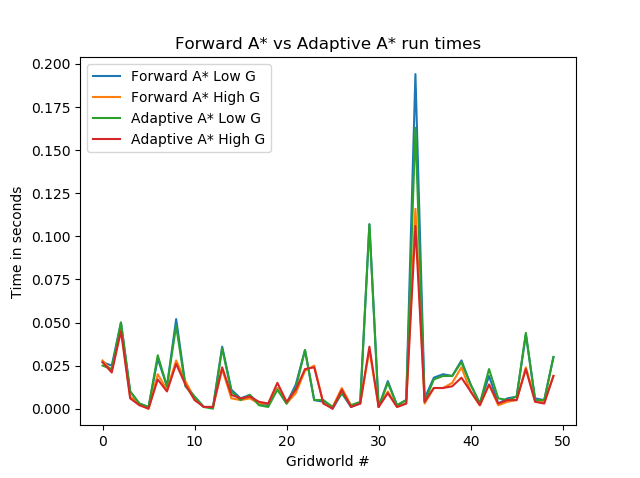
\includegraphics[width=.5\textwidth]{forward_vs_adaptive.png}
		\caption{\label{: }Consistent Heuristic Example}
	\end{figure} 
The results of Forward A star vs Adaptive A star are about as expected. Adaptive A star search utilizes more informed heuristics on each iteration so that it can hopefully waste less resources and time in its attempt to reach the goal cell. On average our Adaptive A star search performed better, but it is still obvious that the Adaptive variation is relying on Forward A star methodologies. Adaptive A star encounters a similar pitfall when trying to find a goal cell that is not actually reachable (although High G tie breaking helps a lot, the same situation as regular Forward A star search).
\newpage
\section*{Memory Issues}
\tab There are several ways to reduce the amount of memory used in computing A* search algorithms. Due to the nature of how easy implementing complex algorithms is in Python, that was the go to programming language we used to complete this project. At the expense of Python's ease of coding, we sacrificed massive amounts of computation time and memory, however. For example, just to store our 101x101 grid in Python required 93,076 bytes or 744,708 bits. The most optimal programming language above the machine level for this type of task would likely be C where we can easily implement a 101x101 grid at the cost of only 1 bit per cell or10,201 total bits (1,276 bytes). If we were to increase our gridworld size to 1001x1001, to simply store that array in Python would require a massive 9,042,100 bytes or just over 9 MB in grid storage alone. Using test case 50, the required size of all stored f values was approximately 2.8 million bytes, and the required size of all stored g values was approximately 64000 bytes. In total netting around 12 MB of required space in a test case that is extremely far from the worst case. In my attempt to replicate Figure 2, but on the scale of 1001x1001 instead of 101x101, I discovered that my computer is no where near powerful enough to finish that amount of computation in a reasonable amount of time. I expect the required memory to be dozens of gigabytes however, almost solely in stored f values. \\ \\
\tab If we were to calculate the largest gridworld that the algorithm can operate on within a memory limit of 4 MBytes, our answer would rely heavily on whether we are considering worst case or not. The average test case for 101x101 grids used about 0.2 MBytes, the worst case using about 1 MByte. In the worst case then, our maximum grid size would be approximately 202x202 (roughly 4x as many cells as 101x101). And for our average case we could justify a gridworld of size 452x452 (roughly 20x as many cells as a 101x101). This is of course assuming your A* search algorithm is written in Python, a highly memory inefficient language. A well written A* program in C can likely store gridworlds of several thousand by several thousand + inside of 4MB.


















\end{document}